\chapter{Security and Maintenance}


\section{Software Security}
Software security is the application of \orange{techniques that assess, mitigate, and protect software systems from vulnerabilities}.

{
\vspace{-\baselineskip}
\noindent
\begin{wrapfigure}{r}{0.3\textwidth}
   \centering
   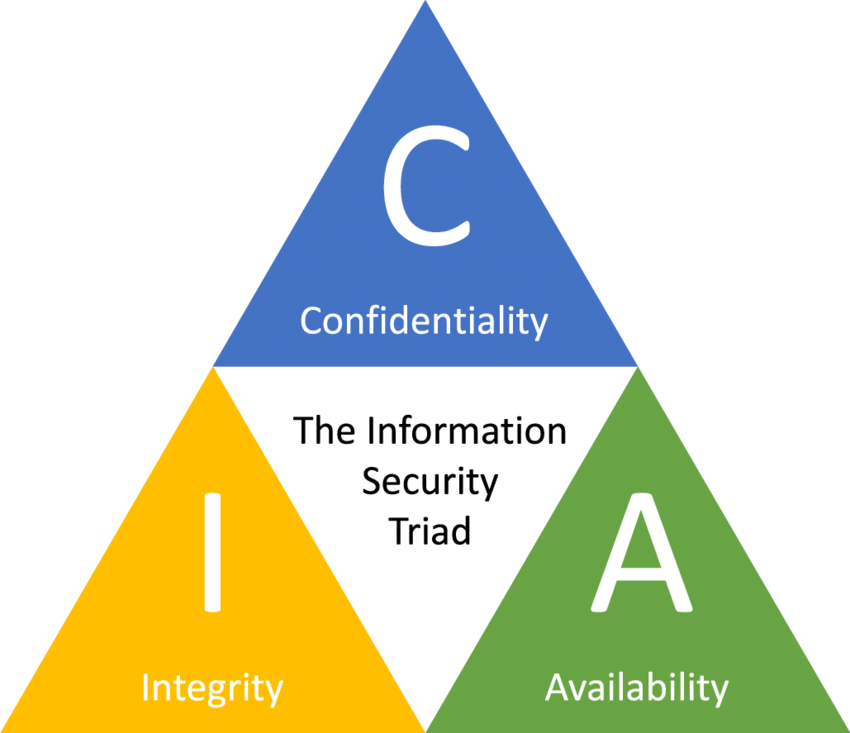
\includegraphics[width=0.25\textwidth]{figures/CIA.png}
 \end{wrapfigure}

\begin{itemize}[parsep=0.5em]
   \item \textbf{Confidentiality:} It protects against disclosure of information to unintended recipients. \textit{Solution:} Encryption, access control, authentication.
   \item \textbf{Integrity:} It allows transferring accurate and correct desired information from senders to intended receivers. \textit{Solution:} Hashing, digital signatures, and checksums.
   \item \textbf{Availability:} It ensures readiness of the information on requirement. \textit{Solution:} \\Redundancy, fault tolerance, backup, regular maintenance, and protection against DDoS attacks.
\end{itemize}
}

\section{Web-based attacks}
\textbf{\textit{Mnemonic:}} 
% I Dare Sneaky Phishers Because Dragons Vomit Purple Acid. Dragons Use Flaming Magic\\
In Dhaka, Smart People Buy Delicious Dumpling Using Fresh Money

\begin{tabularx}{\textwidth}{llX}
   Injection attacks &:& Attacker injects malicious code into a web application and fetch required information. \\
   DNS Spoofing &:& Attacker changes the DNS address of a website to redirect the user to a fake website. \\
   Session Hijacking &:& By stealing the cookies, an attacker can have
   access to all of the user data. \\
   Phishing &:& Steals sensitive information like user credentials and credit card number by pretending to be trustworthy sources. \\
   Brute Force &:& A hacking method that uses trial-and-error to crack passwords, credentials, or encryption keys. \\
   Denial of Service (DOS) &:& Attacker overloads a target server or network with traffic from multiple sources, making it unavailable to legitimate users. \\
   Volume-based attacks &:& Its goal is to saturate the bandwidth of the attacked site, and is measured in bit per second. \\
   Protocol attacks &:& It consumes actual server resources, and is measured in a packet.\\
   Application layer attacks &:& Its goal is to crash the web server and is measured in request per second.\\
   Dictionary attack &:& Attacker uses a list of commonly used passwords to guess original one.\\
   URL Interpretation &:& Attacker changes certain parts of a URL, leading to unauthorized access or data exposure.\\
   File Inclusion Attack &:& Attacker uses the include feature to access sensitive files or run malicious code on the web server.\\
   MITM &:& Attacker to intercepts connection between client and server and acts as a bridge between them.
\end{tabularx}

\section{Security Technologies}
\subsection{Digital Signature}
A digital signature is a mathematical technique which validates the authenticity and integrity of a message, software or digital documents. It allows us to verify the author name, date and time of signatures, and authenticate the message contents. The digital signature offers far more inherent security and intended to solve the problem of tampering and impersonation (Intentionally copy another person's characteristics) in digital communications.

\subsection{Algorithms in Digital Signature}
\begin{itemize}[parsep=0.5em]
   \item \textbf{Key generation algorithm:} The key generation algorithm selects private key randomly from a set of possible private keys. This algorithm provides the private key and its corresponding public key.
   \item \textbf{Signing algorithm:} A signing algorithm produces a signature for the document.
   \item \textbf{Signature verifying algorithm:} A signature verifying algorithm either accepts or rejects the document's authenticity.
\end{itemize}
